% Options for packages loaded elsewhere
\PassOptionsToPackage{unicode}{hyperref}
\PassOptionsToPackage{hyphens}{url}
%
\documentclass[
  12pt,
]{book}
\usepackage{lmodern}
\usepackage{amssymb,amsmath}
\usepackage{ifxetex,ifluatex}
\ifnum 0\ifxetex 1\fi\ifluatex 1\fi=0 % if pdftex
  \usepackage[T1]{fontenc}
  \usepackage[utf8]{inputenc}
  \usepackage{textcomp} % provide euro and other symbols
\else % if luatex or xetex
  \usepackage{unicode-math}
  \defaultfontfeatures{Scale=MatchLowercase}
  \defaultfontfeatures[\rmfamily]{Ligatures=TeX,Scale=1}
\fi
% Use upquote if available, for straight quotes in verbatim environments
\IfFileExists{upquote.sty}{\usepackage{upquote}}{}
\IfFileExists{microtype.sty}{% use microtype if available
  \usepackage[]{microtype}
  \UseMicrotypeSet[protrusion]{basicmath} % disable protrusion for tt fonts
}{}
\makeatletter
\@ifundefined{KOMAClassName}{% if non-KOMA class
  \IfFileExists{parskip.sty}{%
    \usepackage{parskip}
  }{% else
    \setlength{\parindent}{0pt}
    \setlength{\parskip}{6pt plus 2pt minus 1pt}}
}{% if KOMA class
  \KOMAoptions{parskip=half}}
\makeatother
\usepackage{xcolor}
\IfFileExists{xurl.sty}{\usepackage{xurl}}{} % add URL line breaks if available
\IfFileExists{bookmark.sty}{\usepackage{bookmark}}{\usepackage{hyperref}}
\hypersetup{
  pdftitle={ING918XX 系列芯片外设开发者手册},
  pdfauthor={Ingchips Technology Co., Ltd.},
  hidelinks,
  pdfcreator={LaTeX via pandoc}}
\urlstyle{same} % disable monospaced font for URLs
\usepackage{color}
\usepackage{fancyvrb}
\newcommand{\VerbBar}{|}
\newcommand{\VERB}{\Verb[commandchars=\\\{\}]}
\DefineVerbatimEnvironment{Highlighting}{Verbatim}{commandchars=\\\{\}}
% Add ',fontsize=\small' for more characters per line
\usepackage{framed}
\definecolor{shadecolor}{RGB}{248,248,248}
\newenvironment{Shaded}{\begin{snugshade}}{\end{snugshade}}
\newcommand{\AlertTok}[1]{\textcolor[rgb]{0.94,0.16,0.16}{#1}}
\newcommand{\AnnotationTok}[1]{\textcolor[rgb]{0.56,0.35,0.01}{\textbf{\textit{#1}}}}
\newcommand{\AttributeTok}[1]{\textcolor[rgb]{0.77,0.63,0.00}{#1}}
\newcommand{\BaseNTok}[1]{\textcolor[rgb]{0.00,0.00,0.81}{#1}}
\newcommand{\BuiltInTok}[1]{#1}
\newcommand{\CharTok}[1]{\textcolor[rgb]{0.31,0.60,0.02}{#1}}
\newcommand{\CommentTok}[1]{\textcolor[rgb]{0.56,0.35,0.01}{\textit{#1}}}
\newcommand{\CommentVarTok}[1]{\textcolor[rgb]{0.56,0.35,0.01}{\textbf{\textit{#1}}}}
\newcommand{\ConstantTok}[1]{\textcolor[rgb]{0.00,0.00,0.00}{#1}}
\newcommand{\ControlFlowTok}[1]{\textcolor[rgb]{0.13,0.29,0.53}{\textbf{#1}}}
\newcommand{\DataTypeTok}[1]{\textcolor[rgb]{0.13,0.29,0.53}{#1}}
\newcommand{\DecValTok}[1]{\textcolor[rgb]{0.00,0.00,0.81}{#1}}
\newcommand{\DocumentationTok}[1]{\textcolor[rgb]{0.56,0.35,0.01}{\textbf{\textit{#1}}}}
\newcommand{\ErrorTok}[1]{\textcolor[rgb]{0.64,0.00,0.00}{\textbf{#1}}}
\newcommand{\ExtensionTok}[1]{#1}
\newcommand{\FloatTok}[1]{\textcolor[rgb]{0.00,0.00,0.81}{#1}}
\newcommand{\FunctionTok}[1]{\textcolor[rgb]{0.00,0.00,0.00}{#1}}
\newcommand{\ImportTok}[1]{#1}
\newcommand{\InformationTok}[1]{\textcolor[rgb]{0.56,0.35,0.01}{\textbf{\textit{#1}}}}
\newcommand{\KeywordTok}[1]{\textcolor[rgb]{0.13,0.29,0.53}{\textbf{#1}}}
\newcommand{\NormalTok}[1]{#1}
\newcommand{\OperatorTok}[1]{\textcolor[rgb]{0.81,0.36,0.00}{\textbf{#1}}}
\newcommand{\OtherTok}[1]{\textcolor[rgb]{0.56,0.35,0.01}{#1}}
\newcommand{\PreprocessorTok}[1]{\textcolor[rgb]{0.56,0.35,0.01}{\textit{#1}}}
\newcommand{\RegionMarkerTok}[1]{#1}
\newcommand{\SpecialCharTok}[1]{\textcolor[rgb]{0.00,0.00,0.00}{#1}}
\newcommand{\SpecialStringTok}[1]{\textcolor[rgb]{0.31,0.60,0.02}{#1}}
\newcommand{\StringTok}[1]{\textcolor[rgb]{0.31,0.60,0.02}{#1}}
\newcommand{\VariableTok}[1]{\textcolor[rgb]{0.00,0.00,0.00}{#1}}
\newcommand{\VerbatimStringTok}[1]{\textcolor[rgb]{0.31,0.60,0.02}{#1}}
\newcommand{\WarningTok}[1]{\textcolor[rgb]{0.56,0.35,0.01}{\textbf{\textit{#1}}}}
\usepackage{longtable,booktabs}
% Correct order of tables after \paragraph or \subparagraph
\usepackage{etoolbox}
\makeatletter
\patchcmd\longtable{\par}{\if@noskipsec\mbox{}\fi\par}{}{}
\makeatother
% Allow footnotes in longtable head/foot
\IfFileExists{footnotehyper.sty}{\usepackage{footnotehyper}}{\usepackage{footnote}}
\makesavenoteenv{longtable}
\usepackage{graphicx,grffile}
\makeatletter
\def\maxwidth{\ifdim\Gin@nat@width>\linewidth\linewidth\else\Gin@nat@width\fi}
\def\maxheight{\ifdim\Gin@nat@height>\textheight\textheight\else\Gin@nat@height\fi}
\makeatother
% Scale images if necessary, so that they will not overflow the page
% margins by default, and it is still possible to overwrite the defaults
% using explicit options in \includegraphics[width, height, ...]{}
\setkeys{Gin}{width=\maxwidth,height=\maxheight,keepaspectratio}
% Set default figure placement to htbp
\makeatletter
\def\fps@figure{htbp}
\makeatother
\setlength{\emergencystretch}{3em} % prevent overfull lines
\providecommand{\tightlist}{%
  \setlength{\itemsep}{0pt}\setlength{\parskip}{0pt}}
\setcounter{secnumdepth}{5}
\usepackage{booktabs}
\usepackage{longtable}
\usepackage[bf,singlelinecheck=on]{caption}

%\usepackage[bookmarksnumbered]{hyperref}
\hypersetup{bookmarksnumbered=true}

\usepackage[BoldFont,SlantFont,CJKchecksingle]{xeCJK}
\setCJKmonofont{SimSun}% 设置缺省中文字体
%\parindent 2em   %段首缩进

\usepackage[
  top=1cm,
  bottom=1cm,
  left=3cm,
  right=2cm,
  headheight=30pt, % as per the warning by fancyhdr
  includehead,includefoot,
  heightrounded, % to avoid spurious underfull messages
]{geometry}

\usepackage[heading]{ctex}

\usepackage{fancyhdr}
\pagestyle{fancy}
\fancyhead[LO]{
\includegraphics[width=4cm]{./img/logo_en.jpg}}
\fancyhead[RE]{
\includegraphics[width=4cm]{./img/logo_en.jpg}}
%\rhead{\bfseries Result}


%\setmainfont[UprightFeatures={SmallCapsFont=AlegreyaSC-Regular}]{Alegreya}
%\setmainfont[]{Alegreya}
\setmainfont{Liberation Serif}
\setmonofont{Liberation Mono}

\usepackage{framed,color}
\definecolor{shadecolor}{RGB}{248,248,248}

\renewcommand{\textfraction}{0.05}
\renewcommand{\topfraction}{0.8}
\renewcommand{\bottomfraction}{0.8}
\renewcommand{\floatpagefraction}{0.75}

\renewenvironment{quote}{\begin{VF}}{\end{VF}}
\let\oldhref\href
\renewcommand{\href}[2]{#2\footnote{\url{#1}}}

\ifxetex
  \usepackage{letltxmacro}
  \setlength{\XeTeXLinkMargin}{1pt}
  \LetLtxMacro\SavedIncludeGraphics\includegraphics
  \def\includegraphics#1#{% #1 catches optional stuff (star/opt. arg.)
    \IncludeGraphicsAux{#1}%
  }%
  \newcommand*{\IncludeGraphicsAux}[2]{%
    \XeTeXLinkBox{%
      \SavedIncludeGraphics#1{#2}%
    }%
  }%
\fi

\makeatletter
\newenvironment{kframe}{%
\medskip{}
\setlength{\fboxsep}{.8em}
 \def\at@end@of@kframe{}%
 \ifinner\ifhmode%
  \def\at@end@of@kframe{\end{minipage}}%
  \begin{minipage}{\columnwidth}%
 \fi\fi%
 \def\FrameCommand##1{\hskip\@totalleftmargin \hskip-\fboxsep
 \colorbox{shadecolor}{##1}\hskip-\fboxsep
     % There is no \\@totalrightmargin, so:
     \hskip-\linewidth \hskip-\@totalleftmargin \hskip\columnwidth}%
 \MakeFramed {\advance\hsize-\width
   \@totalleftmargin\z@ \linewidth\hsize
   \@setminipage}}%
 {\par\unskip\endMakeFramed%
 \at@end@of@kframe}
\makeatother

\makeatletter
\@ifundefined{Shaded}{
}{\renewenvironment{Shaded}{\begin{kframe}}{\end{kframe}}}
\makeatother

\newenvironment{rmdblock}[1]
  {
  \begin{itemize}
  \renewcommand{\labelitemi}{
    \raisebox{-.7\height}[0pt][0pt]{
      {\setkeys{Gin}{width=3em,keepaspectratio}\includegraphics{images/#1}}
    }
  }
  \setlength{\fboxsep}{1em}
  \begin{kframe}
  \item
  }
  {
  \end{kframe}
  \end{itemize}
  }
\newenvironment{rmdnote}
  {\begin{rmdblock}{note}}
  {\end{rmdblock}}
\newenvironment{rmdcaution}
  {\begin{rmdblock}{caution}}
  {\end{rmdblock}}
\newenvironment{rmdimportant}
  {\begin{rmdblock}{important}}
  {\end{rmdblock}}
\newenvironment{rmdtip}
  {\begin{rmdblock}{tip}}
  {\end{rmdblock}}
\newenvironment{rmdwarning}
  {\begin{rmdblock}{warning}}
  {\end{rmdblock}}

\usepackage{makeidx}
\makeindex

\urlstyle{tt}

\usepackage{amsthm}
\makeatletter
\def\thm@space@setup{%
  \thm@preskip=8pt plus 2pt minus 4pt
  \thm@postskip=\thm@preskip
}
\makeatother

\frontmatter

\let\oldmaketitle\maketitle
\AtBeginDocument{\let\maketitle\relax}

% % Definition of \maketitle
% \makeatletter
%     \begin{titlepage}
%         \begin{center}
%             
\includegraphics[width=0.7\linewidth]{./img/logo_en.jpg}\\[4ex]
%             {\huge \bfseries  \@title }\\[2ex]
%             {\LARGE  \@author}\\[50ex]
%             {\large \@date}
%         \end{center}
%     \end{titlepage}
% \makeatother
\usepackage[]{natbib}
\bibliographystyle{apalike}

\title{ING918XX 系列芯片外设开发者手册}
\author{Ingchips Technology Co., Ltd.}
\date{}

\begin{document}
\maketitle

%\cleardoublepage\newpage\thispagestyle{empty}\null
%\cleardoublepage\newpage\thispagestyle{empty}\null
%\cleardoublepage\newpage
\thispagestyle{empty}
\begin{center}
\end{center}

\setlength{\abovedisplayskip}{-5pt}
\setlength{\abovedisplayshortskip}{-5pt}

\thispagestyle{empty}

\makeatletter
\begin{center}
    \vspace{5ex}
    
\includegraphics{./img/logo_en.jpg}\\[15ex]
    {\huge  \@title }
    \noindent\rule{10cm}{0.4pt}\\[68ex]
    %{\LARGE  \@author}\\[60ex] 
    {\large \@author}
\end{center}
\makeatother


\newpage
\thispagestyle{empty}

%\let\maketitle\oldmaketitle
%\maketitle

{
\setcounter{tocdepth}{3}
\tableofcontents
}
\listoftables
\listoffigures
\mainmatter

\hypertarget{revision-history}{%
\chapter{版本历史}\label{revision-history}}

\begin{longtable}[]{@{}lll@{}}
\toprule
版本 & 信息 & 日期\tabularnewline
\midrule
\endhead
0.1 & 初始版本 & 2022-xx-xx\tabularnewline
\bottomrule
\end{longtable}

\hypertarget{ch-overview}{%
\chapter{概览}\label{ch-overview}}

欢迎使用 \emph{INGCHIPS} 918xx/916xx 软件开发工具包 (SDK).

ING918XX 系列芯片支持蓝牙 5.0/5.1 规范,内置高性能 32bit RISC MCU、Flash,以及丰富的外设、
高性能低功耗 BLE RF 收发机。BLE 发射功率。

本文介绍 SoC 外设及其开发方法。每个章节介绍一种外设,各种外设与芯片数据手册之外设一一对应,
基于 API 的兼容性、避免误解等因素,存在以下例外:

\begin{itemize}
\tightlist
\item
  PINCTRL 对应于数据手册之 IOMUX
\item
  SYSCTRL 是一个``虚拟''外设,负责管理各种 SoC 功能,组合了几种相关的硬件模块
\end{itemize}

SDK 外设驱动的源代码开放,其中包含很多常数,而且几乎没有注释 ------ 这是有意为之,开发者只需要关注头文件,而不要尝试修改源代码。

918xx系列分为9187和9188两个子系列,9187和9188各自根据封装不同而有不同的后缀。9187与9188的区别在于9188是5.1规范,
而9187是5.0规范。对于软件开发者来说,如果需要5.1规范则需要将sdk运行于9188系列的芯片上,如开发AOA等功能。

总而言之,9188向下兼容9187,两者共用一套sdk,开放给开发者的寄存器及接口均是一致的。

\hypertarget{ux7f29ux7565ux8bedux53caux672fux8bed}{%
\section{缩略语及术语}\label{ux7f29ux7565ux8bedux53caux672fux8bed}}

\begin{longtable}[]{@{}cl@{}}
\caption{\label{tab:ch0-abbreviations} 缩略语}\tabularnewline
\toprule
缩略语 & 说明\tabularnewline
\midrule
\endfirsthead
\toprule
缩略语 & 说明\tabularnewline
\midrule
\endhead
ADC & 模数转换器(Analog-to-Digital Converter)\tabularnewline
FIFO & 先进先出队列(First In First Out)\tabularnewline
GPIO & 通用输入输出(General-Purpose Input/Output)\tabularnewline
I2C & 集成电路间总线(Inter-Integrated Circuit)\tabularnewline
PWM & 脉宽调制信号(Pulse Width Modulation)\tabularnewline
QDEC & 正交解码器(Quadrature Decoder)\tabularnewline
RTC & 实时时钟(Real-time Clock)\tabularnewline
SPI & 串行外设接口(Serial Peripheral Interface)\tabularnewline
UART & 通用异步收发器(Universal Asynchronous Receiver/Transmitter)\tabularnewline
\#\# 参考文档 &\tabularnewline
\bottomrule
\end{longtable}

\begin{enumerate}
\def\labelenumi{\arabic{enumi}.}
\tightlist
\item
  Bluetooth SIG\footnote{\url{https://www.bluetooth.com/}}
\item
  ING918XX 系列芯片数据手册
\end{enumerate}

\hypertarget{ux901aux7528ux8f93ux5165ux8f93ux51fagpio}{%
\chapter{通用输入输出(GPIO)}\label{ux901aux7528ux8f93ux5165ux8f93ux51fagpio}}

\hypertarget{ux529fux80fdux6982ux8ff0}{%
\section{功能概述}\label{ux529fux80fdux6982ux8ff0}}

GPIO 模块常用于驱动 LED 或者其它指示器,控制片外设备,感知数字信号输入,检测信号边沿,
或者从低功耗状态唤醒系统。ING918XX 系列芯片内部支持最多 20 个 GPIO,通过 \protect\hyperlink{ch-pinctrl}{PINCTRL}
可将 GPIO \(n\) 引出到芯片 IO 管脚 \(n\)。

特性:

\begin{itemize}
\tightlist
\item
  每个 GPIO 都可单独配置为输入或输出
\item
  每个 GPIO 都可作为中断请求,中断触发方式支持边沿触发(上升、下降单沿触发,或者双沿触发)
  和电平触发(高电平或低电平)
\end{itemize}

\hypertarget{ux4f7fux7528ux8bf4ux660e}{%
\section{使用说明}\label{ux4f7fux7528ux8bf4ux660e}}

\hypertarget{ux8bbeux7f6e-io-ux65b9ux5411}{%
\subsection{设置 IO 方向}\label{ux8bbeux7f6e-io-ux65b9ux5411}}

在使用 GPIO 之前先按需要配置 IO 方向:

\begin{itemize}
\tightlist
\item
  需要用于输出信号时:配置为输出
\item
  需要用于读取信号时:配置为输入
\item
  需要用于生产中断请求时:配置为输入
\item
  需要高阻态时:配置为高阻态
\end{itemize}

使用 \texttt{GIO\_SetDirection} 配置 GPIO 的方向。GPIO 支持四种方向:

\begin{Shaded}
\begin{Highlighting}[]
\KeywordTok{typedef} \KeywordTok{enum}
\NormalTok{\{}
\NormalTok{    GIO_DIR_INPUT,  }\CommentTok{// 输入}
\NormalTok{    GIO_DIR_OUTPUT, }\CommentTok{// 输出}
\NormalTok{    GIO_DIR_BOTH,   }\CommentTok{// 同时支持输入、输出}
\NormalTok{    GIO_DIR_NONE    }\CommentTok{// 高阻态}
\NormalTok{\} GIO_Direction_t;}
\end{Highlighting}
\end{Shaded}

\begin{rmdcaution}
如无必要,不要使用 \texttt{GIO\_DIR\_BOTH}。
\end{rmdcaution}

\hypertarget{ux8bfbux53d6ux8f93ux5165}{%
\subsection{读取输入}\label{ux8bfbux53d6ux8f93ux5165}}

使用 \texttt{GIO\_ReadValue} 读取某个 GPIO 当前输入的电平信号,例如读取 GPIO 0 的输入:

\begin{Shaded}
\begin{Highlighting}[]
\DataTypeTok{uint8_t}\NormalTok{ value = GIO_ReadValue(GIO_GPIO_0);}
\end{Highlighting}
\end{Shaded}

使用 \texttt{GIO\_ReadAll} 可以同时读取所有 GPIO 当前输入的电平信号。其返回值的第 \(n\) 比特
(第 0 比特为最低比特)对应 GPIO \(n\) 的输入;如果 GPIO \(n\) 当前不支持输入,那么第 \(n\)
比特为 0:

\begin{Shaded}
\begin{Highlighting}[]
\DataTypeTok{uint64_t}\NormalTok{ GIO_ReadAll(}\DataTypeTok{void}\NormalTok{);}
\end{Highlighting}
\end{Shaded}

\hypertarget{ux8bbeux7f6eux8f93ux51fa}{%
\subsection{设置输出}\label{ux8bbeux7f6eux8f93ux51fa}}

使用 \texttt{GIO\_WriteValue} 设置某个 GPIO 输出的电平信号,例如使 GPIO 0 输出高电平(1):

\begin{Shaded}
\begin{Highlighting}[]
\NormalTok{GIO_WriteValue(GIO_GPIO_0, }\DecValTok{1}\NormalTok{);}
\end{Highlighting}
\end{Shaded}

\hypertarget{ux914dux7f6eux4e2dux65adux8bf7ux6c42}{%
\subsection{配置中断请求}\label{ux914dux7f6eux4e2dux65adux8bf7ux6c42}}

使用 \texttt{GIO\_ConfigIntSource} 配置 GPIO 生成中断请求。

\begin{Shaded}
\begin{Highlighting}[]
\DataTypeTok{void}\NormalTok{ GIO_ConfigIntSource(}
  \DataTypeTok{const}\NormalTok{ GIO_Index_t io_index,     }\CommentTok{// GPIO 编号}
  \DataTypeTok{const} \DataTypeTok{uint8_t}\NormalTok{ enable,           }\CommentTok{// 使能的边沿或者电平类型组合}
  \DataTypeTok{const}\NormalTok{ GIO_IntTriggerType_t type }\CommentTok{// 触发类型}
\NormalTok{  );}
\end{Highlighting}
\end{Shaded}

其中的 \texttt{enable} 为以下两个值的组合(0 表示禁止产生中断请求):

\begin{Shaded}
\begin{Highlighting}[]
\KeywordTok{typedef} \KeywordTok{enum}
\NormalTok{\{}
\NormalTok{    ...LOGIC_LOW_OR_FALLING_EDGE = ..., }\CommentTok{// 低电平或者下降沿}
\NormalTok{    ...LOGIC_HIGH_OR_RISING_EDGE = ...  }\CommentTok{// 高电平或者上升沿}
\NormalTok{\} GIO_IntTriggerEnable_t;}
\end{Highlighting}
\end{Shaded}

触发类型有两种:

\begin{Shaded}
\begin{Highlighting}[]
\KeywordTok{typedef} \KeywordTok{enum}
\NormalTok{\{}
\NormalTok{    GIO_INT_EDGE,   }\CommentTok{// 边沿触发}
\NormalTok{    GIO_INT_LOGIC   }\CommentTok{// 电平触发}
\NormalTok{\} GIO_IntTriggerType_t;}
\end{Highlighting}
\end{Shaded}

\begin{itemize}
\item
  例如将 GPIO 0 配置为上升沿触发中断

\begin{Shaded}
\begin{Highlighting}[]
\NormalTok{GIO_ConfigIntSource(GIO_GPIO_0,}
\NormalTok{  ...LOGIC_HIGH_OR_RISING_EDGE,}
\NormalTok{  GIO_INT_EDGE);}
\end{Highlighting}
\end{Shaded}
\item
  例如将 GPIO 0 配置为双沿触发中断

\begin{Shaded}
\begin{Highlighting}[]
\NormalTok{GIO_ConfigIntSource(GIO_GPIO_0,}
\NormalTok{  ...LOGIC_HIGH_OR_RISING_EDGE | ..._HIGH_OR_RISING_EDGE,}
\NormalTok{  GIO_INT_EDGE);}
\end{Highlighting}
\end{Shaded}
\item
  例如将 GPIO 0 配置为高电平触发

\begin{Shaded}
\begin{Highlighting}[]
\NormalTok{GIO_ConfigIntSource(GIO_GPIO_0,}
\NormalTok{  ...LOGIC_HIGH_OR_RISING_EDGE,}
\NormalTok{  GIO_INT_LOGIC);}
\end{Highlighting}
\end{Shaded}
\end{itemize}

\hypertarget{ux5904ux7406ux4e2dux65adux72b6ux6001}{%
\subsection{处理中断状态}\label{ux5904ux7406ux4e2dux65adux72b6ux6001}}

在用 \texttt{platform\_set\_irq\_callback} 注册好GPIO中断回调函数后,在中断里用 \texttt{GIO\_GetIntStatus} 可获取某个 GPIO 上的中断触发状态,返回非 0 值表示该 GPIO
上产生了中断请求;用 \texttt{GIO\_GetAllIntStatus} 一次性获取所有 GPIO 的中断触发状态,
第 \(n\) 比特(第 0 比特为最低比特)对应 GPIO \(n\) 上的中断触发状态。

GPIO 产生中断后,需要消除中断状态方可再次触发。用 \texttt{GIO\_ClearIntStatus} 消除某个 GPIO
上中断状态,用 \texttt{GIO\_ClearAllIntStatus} 一次性清除所有 GPIO 上可能存在的中断触发状态。

\hypertarget{i2cux529fux80fdux6982ux8ff0}{%
\chapter{I2C功能概述}\label{i2cux529fux80fdux6982ux8ff0}}

\begin{itemize}
\tightlist
\item
  两个I2C模块
\item
  支持Master/Slave模式
\item
  支持7bit/10bit地址
\item
  支持DMA和QUEUE模式
\end{itemize}

\hypertarget{i2cux4f7fux7528ux8bf4ux660e}{%
\section{I2C使用说明}\label{i2cux4f7fux7528ux8bf4ux660e}}

以下场景中均以I2C0为例,如果需要I2C1则可以根据情况修改

\hypertarget{ux4f7fux7528ux65b9ux6cd5}{%
\section{使用方法}\label{ux4f7fux7528ux65b9ux6cd5}}

\hypertarget{masterux8bfbux4e9bux91c7ux7528queueux6a21ux5f0f}{%
\subsection{Master读些,采用QUEUE模式}\label{masterux8bfbux4e9bux91c7ux7528queueux6a21ux5f0f}}

\begin{Shaded}
\begin{Highlighting}[]
\PreprocessorTok{#define I2C_PORT        I2C_PORT_0}
\PreprocessorTok{#define I2C_ADDR        0X76}
\end{Highlighting}
\end{Shaded}

\hypertarget{ux6253ux5f00i2cux65f6ux949f}{%
\subsubsection{打开I2C时钟}\label{ux6253ux5f00i2cux65f6ux949f}}

\begin{Shaded}
\begin{Highlighting}[]
\NormalTok{    SYSCTRL_ClearClkGateMulti( (}\DecValTok{1}\NormalTok{ << SYSCTRL_ClkGate_APB_I2C0)}
\NormalTok{                              |(}\DecValTok{1}\NormalTok{ << SYSCTRL_ClkGate_APB_PinCtrl));}
\end{Highlighting}
\end{Shaded}

\hypertarget{ux914dux7f6ei2cux7684ioux53e3}{%
\subsubsection{配置I2C的IO口}\label{ux914dux7f6ei2cux7684ioux53e3}}

\begin{Shaded}
\begin{Highlighting}[]
\NormalTok{    PINCTRL_SetPadMux(}\DecValTok{10}\NormalTok{, IO_SOURCE_I2C0_SCL_O);}
\NormalTok{    PINCTRL_SetPadMux(}\DecValTok{11}\NormalTok{, IO_SOURCE_I2C0_SDO);}
\NormalTok{    PINCTRL_SelI2cSclIn(I2C_PORT, }\DecValTok{10}\NormalTok{);}
\end{Highlighting}
\end{Shaded}

\hypertarget{i2cux6a21ux5757ux521dux59cbux5316}{%
\subsubsection{I2C模块初始化}\label{i2cux6a21ux5757ux521dux59cbux5316}}

\begin{Shaded}
\begin{Highlighting}[]
\NormalTok{I2C_CTRL0_CLR(I2C_BASE(I2C_PORT), I2C_CTRL0_SFTRST | I2C_CTRL0_CLKGATE);}
\end{Highlighting}
\end{Shaded}

\hypertarget{i2cux5199ux64cdux4f5c}{%
\subsubsection{I2C写操作}\label{i2cux5199ux64cdux4f5c}}

\begin{Shaded}
\begin{Highlighting}[]
\DataTypeTok{int}\NormalTok{ i2c_do_write(}\DataTypeTok{const}\NormalTok{ i2c_port_t port, }\DataTypeTok{const} \DataTypeTok{uint32_t}\NormalTok{ nrm, }\DataTypeTok{uint8_t}\NormalTok{ addr, }\DataTypeTok{const} \DataTypeTok{uint8_t}\NormalTok{ *byte_data, }\DataTypeTok{int16_t}\NormalTok{ length)}
\NormalTok{\{}
    \DataTypeTok{uint32_t}\NormalTok{ *p_data = (}\DataTypeTok{uint32_t}\NormalTok{ *)(byte_data + }\DecValTok{3}\NormalTok{);}
    \DataTypeTok{uint32_t}\NormalTok{ data = (addr <<  }\DecValTok{1}\NormalTok{) | }\DecValTok{0}\NormalTok{;     }\CommentTok{// control: write}
\NormalTok{    I2C_TypeDef *BASE = I2C_BASE(port);}
    \DataTypeTok{int}\NormalTok{ timeout = I2C_HW_TIME_OUT;}

    \ControlFlowTok{if}\NormalTok{ (length > }\DecValTok{0}\NormalTok{)}
\NormalTok{        data |= (byte_data[}\DecValTok{0}\NormalTok{] <<  }\DecValTok{8}\NormalTok{) | (byte_data[}\DecValTok{1}\NormalTok{] << }\DecValTok{16}\NormalTok{) | (byte_data[}\DecValTok{2}\NormalTok{] << }\DecValTok{24}\NormalTok{);}

\NormalTok{    I2C_CTRL0_CLR(BASE, I2C_CTRL0_SFTRST | I2C_CTRL0_CLKGATE);}

    \CommentTok{// ONLY SUPPORT PIO QUEUE MODE, SET HW_I2C_QUEUECTRL_PIO_QUEUE_MODE AT FRIST}
\NormalTok{    I2C_QUEUECTRL_SET(BASE, I2C_QUEUECTRL_PIO_QUEUE_MODE);}

    \CommentTok{// frist operation, do not need clear I2C_QUEUECTRL and I2C_QUEUECMD.}
\NormalTok{    BASE->I2C_QUEUECMD.NRM = nrm + }\DecValTok{1}\NormalTok{ + length;}

\NormalTok{    I2C_QUEUECTRL_SET(BASE, I2C_QUEUECTRL_QUEUE_RUN);}


\NormalTok{    length += }\DecValTok{1}\NormalTok{;}
    \ControlFlowTok{while}\NormalTok{ (}\DecValTok{1}\NormalTok{)}
\NormalTok{    \{}
\NormalTok{        while_with_timeout(I2C_QUEUESTAT_WR_QUEUE_FULL(BASE));}
\NormalTok{        BASE->I2C_DATA = data;}
\NormalTok{        length -= }\DecValTok{4}\NormalTok{;}
        \ControlFlowTok{if}\NormalTok{ (length <= }\DecValTok{0}\NormalTok{)}
            \ControlFlowTok{break}\NormalTok{;}
\NormalTok{        data = *p_data;}
\NormalTok{        p_data++;}
\NormalTok{    \}}

    \CommentTok{// WAIT I2C_CTRL1_DATA_ENGINE_CMPLT_IRQ (software polling)}
\NormalTok{    while_with_timeout(GET_I2C_CTRL1_DATA_ENGINE_CMPLT_IRQ(BASE) == }\DecValTok{0}\NormalTok{);}
\NormalTok{    I2C_CTRL1_CLR(BASE, I2C_CTRL1_DATA_ENGINE_CMPLT_IRQ);}

    \CommentTok{// }\AlertTok{NOTE}\CommentTok{ : MUST SET I2C_QUEUECTRL_WR_CLEAR}
\NormalTok{    I2C_QUEUECTRL_SET(BASE, I2C_QUEUECTRL_WR_CLEAR);}
\NormalTok{    I2C_QUEUECTRL_CLR(BASE, I2C_QUEUECTRL_WR_CLEAR);}

    \ControlFlowTok{return} \DecValTok{0}\NormalTok{;}
\NormalTok{\}}
\end{Highlighting}
\end{Shaded}

\hypertarget{i2cux8bfbux64cdux4f5c}{%
\subsubsection{I2C读操作}\label{i2cux8bfbux64cdux4f5c}}

\begin{Shaded}
\begin{Highlighting}[]
\DataTypeTok{int}\NormalTok{ i2c_read(}\DataTypeTok{const}\NormalTok{ i2c_port_t port, }\DataTypeTok{uint8_t}\NormalTok{ addr,}
              \DataTypeTok{const} \DataTypeTok{uint8_t}\NormalTok{ *write_data, }\DataTypeTok{int16_t}\NormalTok{ write_len,}
              \DataTypeTok{uint8_t}\NormalTok{ *read_data, }\DataTypeTok{int16_t}\NormalTok{ read_length)}
\NormalTok{\{}
\NormalTok{    I2C_TypeDef *BASE = I2C_BASE(port);}
    \DataTypeTok{int}\NormalTok{ timeout = I2C_HW_TIME_OUT;}

    \ControlFlowTok{if}\NormalTok{ (write_len)}
\NormalTok{    \{}
        \CommentTok{// STEP 1: send write command}
        \DataTypeTok{int}\NormalTok{ r = i2c_do_write(port, I2C_QUEUECMD_PRE_SEND_START | I2C_QUEUECMD_MASTER_MODE | I2C_QUEUECMD_DIRECTION,}
\NormalTok{                     addr, write_data, write_len);}
        \ControlFlowTok{if}\NormalTok{ (r != }\DecValTok{0}\NormalTok{) }\ControlFlowTok{return}\NormalTok{ r;}
\NormalTok{    \}}
    \ControlFlowTok{else}
\NormalTok{    \{}
\NormalTok{        I2C_CTRL0_CLR(BASE, I2C_CTRL0_SFTRST | I2C_CTRL0_CLKGATE);}

        \CommentTok{// ONLY SUPPORT PIO QUEUE MODE, SET HW_I2C_QUEUECTRL_PIO_QUEUE_MODE AT FRIST}
\NormalTok{        I2C_QUEUECTRL_SET(BASE, I2C_QUEUECTRL_PIO_QUEUE_MODE);}
\NormalTok{    \}}

    \CommentTok{// STEP 2 : transmit (control byte + Read command), need hold SCL (I2C_QUEUECMD_RETAIN_CLOCK)}
\NormalTok{    BASE->I2C_QUEUECMD.NRM = (I2C_QUEUECMD_RETAIN_CLOCK | I2C_QUEUECMD_PRE_SEND_START | I2C_QUEUECMD_MASTER_MODE | I2C_QUEUECMD_DIRECTION |}
          \DecValTok{1}\NormalTok{);}

\NormalTok{    I2C_QUEUECTRL_SET(BASE, I2C_QUEUECTRL_QUEUE_RUN);}

\NormalTok{    BASE->I2C_DATA = }\BaseNTok{0xA5}\BuiltInTok{UL}\NormalTok{ << }\DecValTok{24}\NormalTok{ | }\BaseNTok{0x5A}\NormalTok{   << }\DecValTok{16}\NormalTok{ |}\BaseNTok{0xAA}\NormalTok{   <<  }\DecValTok{8}\NormalTok{ | (addr <<  }\DecValTok{1}\NormalTok{) | }\DecValTok{1}\NormalTok{;}

\NormalTok{    while_with_timeout(GET_I2C_CTRL1_DATA_ENGINE_CMPLT_IRQ(BASE) == }\DecValTok{0}\NormalTok{);}

    \CommentTok{// CLEAR I2C_CTRL1_DATA_ENGINE_CMPLT_IRQ}
\NormalTok{    I2C_CTRL1_CLR(BASE, I2C_CTRL1_DATA_ENGINE_CMPLT_IRQ);}

    \CommentTok{// }\AlertTok{NOTE}\CommentTok{ : MUST SET I2C_QUEUECTRL_WR_CLEAR}
\NormalTok{    I2C_QUEUECTRL_SET(BASE, I2C_QUEUECTRL_WR_CLEAR);}
\NormalTok{    I2C_QUEUECTRL_CLR(BASE, I2C_QUEUECTRL_WR_CLEAR);}


    \CommentTok{//}
    \CommentTok{// STEP 3 : read data byte + (NO ACK) + STOP}
    \CommentTok{//}

\NormalTok{    BASE->I2C_QUEUECMD.NRM = (I2C_QUEUECMD_SEND_NAK_ON_LAST | I2C_QUEUECMD_POST_SEND_STOP | I2C_QUEUECMD_MASTER_MODE |}
         \CommentTok{/*I2C_QUEUECMD_XFER_COUNT*/}
\NormalTok{         read_length);}

\NormalTok{    I2C_QUEUECTRL_SET(BASE, I2C_QUEUECTRL_QUEUE_RUN);}

    \CommentTok{// Receive DATA use I2C_QUEUEDATA;}
    \ControlFlowTok{while}\NormalTok{ (read_length > }\DecValTok{0}\NormalTok{)}
\NormalTok{    \{}
        \CommentTok{// check whether rdFIFO is empty}
\NormalTok{        while_with_timeout(I2C_QUEUESTAT_RD_QUEUE_EMPTY(BASE));}

        \DataTypeTok{int}\NormalTok{ len = write_bytes(read_data, BASE->I2C_QUEUEDATA, read_length);}
\NormalTok{        read_data += len;}
\NormalTok{        read_length -= len;}
\NormalTok{    \}}

    \CommentTok{// WAIT I2C_CTRL1_DATA_ENGINE_CMPLT_IRQ (software polling)}
\NormalTok{    while_with_timeout(GET_I2C_CTRL1_DATA_ENGINE_CMPLT_IRQ(BASE) == }\DecValTok{0}\NormalTok{);}

    \CommentTok{// cLEAR I2C_CTRL1_DATA_ENGINE_CMPLT_IRQ}
\NormalTok{    I2C_CTRL1_CLR(BASE, I2C_CTRL1_DATA_ENGINE_CMPLT_IRQ);}

    \CommentTok{// }\AlertTok{NOTE}\CommentTok{ : CLEAR I2C_QUEUECTRL_RD_CLEAR}
\NormalTok{    I2C_QUEUECTRL_SET(BASE, I2C_QUEUECTRL_RD_CLEAR);}
\NormalTok{    I2C_QUEUECTRL_CLR(BASE, I2C_QUEUECTRL_RD_CLEAR);}


    \ControlFlowTok{return} \DecValTok{0}\NormalTok{;}
\NormalTok{\}}
\end{Highlighting}
\end{Shaded}

\hypertarget{ch-pinctrl}{%
\chapter{管脚管理(PINCTRL)}\label{ch-pinctrl}}

\hypertarget{ux529fux80fdux6982ux8ff0-1}{%
\section{功能概述}\label{ux529fux80fdux6982ux8ff0-1}}

PINCTRL 模块管理芯片所有 IO 管脚的功能,包括外设 IO 的映射,上拉、下拉选择,输入模式控制,
输出驱动能力设置等。

IO管脚特性如下:

\begin{itemize}
\tightlist
\item
  每个 IO 管脚可以映射多种不同功能的外设
\item
  每个 IO 管脚都支持上拉或下拉
\item
  每个 IO 管脚都支持施密特触发输入方式
\item
  每个 IO 管脚支持四种输出驱动能力
\end{itemize}

鉴于片内外设丰富、IO 管脚多,进行管脚全映射并不现实,为此,PINCTRL 尽量保证灵活性的前提下做了一定取舍、优化。
部分常用外设的输入、输出功能管脚可与 \(\{{0-19\}}\) 这 20 个常用 IO 之间任意连接(全映射),
这部分常用外设功能管脚总结于表 \ref{tab:ch-pinctrl-common-set}。
表 \ref{tab:ch-pinctrl-mapping} 列出了其它外设功能管脚支持映射到哪些 IO 管脚上。

\begin{longtable}[]{@{}ll@{}}
\caption{\label{tab:ch-pinctrl-common-set} 支持与常用 IO 全映射的常用功能管脚}\tabularnewline
\toprule
外设 & 功能管脚\tabularnewline
\midrule
\endfirsthead
\toprule
外设 & 功能管脚\tabularnewline
\midrule
\endhead
I2C0 & I2C0\_SCL\_O, I2C0\_SDO\tabularnewline
I2C1 & I2C1\_SCL\_O, I2C1\_SDO\tabularnewline
SPI0 & SPI0\_CLK, SPI0\_DO, SPI0\_SSN\tabularnewline
SPI1 & SPI1\_CLK, SPI1\_DO, SPI1\_SSN\tabularnewline
UART0 & UART0\_TXD, UART0\_RTS\tabularnewline
UART1 & UART1\_TXD, UART1\_RTS\tabularnewline
\bottomrule
\end{longtable}

\begin{longtable}[]{@{}ll@{}}
\caption{\label{tab:ch-pinctrl-mapping} 其它外设功能管脚的映射关系}\tabularnewline
\toprule
外设功能管脚 & 可连接到的 IO 管脚\tabularnewline
\midrule
\endfirsthead
\toprule
外设功能管脚 & 可连接到的 IO 管脚\tabularnewline
\midrule
\endhead
PWM\_0A & 0-11\tabularnewline
PWM\_0B & 0-11\tabularnewline
PWM\_1A & 0-11\tabularnewline
PWM\_1B & 0-11\tabularnewline
PWM\_2A & 0-11\tabularnewline
PWM\_2B & 0-11\tabularnewline
PWM\_3A & 0-11\tabularnewline
PWM\_3B & 0-11\tabularnewline
PWM\_4A & 0-11\tabularnewline
PWM\_4B & 0-11\tabularnewline
PWM\_5A & 0-11\tabularnewline
PWM\_5B & 0-11\tabularnewline
\bottomrule
\end{longtable}

\hypertarget{ux4f7fux7528ux8bf4ux660e-1}{%
\section{使用说明}\label{ux4f7fux7528ux8bf4ux660e-1}}

\hypertarget{ux4e3aux5916ux8bbeux914dux7f6e-io-ux7ba1ux811a}{%
\subsection{为外设配置 IO 管脚}\label{ux4e3aux5916ux8bbeux914dux7f6e-io-ux7ba1ux811a}}

\begin{enumerate}
\def\labelenumi{\arabic{enumi}.}
\item
  将外设输出连接到 IO 管脚

  通过 \texttt{PINCTRL\_SetPadMux} 将外设输出连接到 IO 管脚。
  注意按照表 \ref{tab:ch-pinctrl-common-set} 和 表 \ref{tab:ch-pinctrl-mapping}
  确认硬件是否支持。对于不支持的配置,显然无法生效。

\begin{Shaded}
\begin{Highlighting}[]
\DataTypeTok{void}\NormalTok{ PINCTRL_SetPadMux(}
  \DataTypeTok{const} \DataTypeTok{uint8_t}\NormalTok{ io_pin_index, }\CommentTok{// IO 序号 (0..19)}
  \DataTypeTok{const}\NormalTok{ io_source_t source    }\CommentTok{// IO 源}
\NormalTok{);}
\end{Highlighting}
\end{Shaded}
\item
  将 IO 管脚连接到外设的输入

  对于有些外设的输入同样通过 \texttt{PINCTRL\_SetPadMux} 配置。对于另一些输入,
  PINCTRL 为不同的外设分别提供了 API 用以配置输入。比如对于 UART 用于硬件流控的
  RXD,需要通过 \texttt{PINCTRL\_SelUartRxdIn} 配置 :

\begin{Shaded}
\begin{Highlighting}[]
\DataTypeTok{void}\NormalTok{ PINCTRL_SelUartRxdIn(}
    \DataTypeTok{const}\NormalTok{ uart_port_t port, }\CommentTok{//UART 序号}
    \DataTypeTok{const} \DataTypeTok{uint8_t}\NormalTok{ io_pin_index)}\CommentTok{//连接到 RXD 输入的 IO 管脚}
\end{Highlighting}
\end{Shaded}
\end{enumerate}

\hypertarget{ux914dux7f6eux4e0bux62c9ux4e0bux62c9}{%
\subsection{配置下拉、下拉}\label{ux914dux7f6eux4e0bux62c9ux4e0bux62c9}}

IO 管脚的上拉、下拉模式通过 \texttt{PINCTRL\_Pull} 配置:

\begin{Shaded}
\begin{Highlighting}[]
\DataTypeTok{void}\NormalTok{ PINCTRL_Pull(}
  \DataTypeTok{const} \DataTypeTok{uint8_t}\NormalTok{ io_pin_index,     }\CommentTok{// IO 管脚序号}
  \DataTypeTok{const}\NormalTok{ pinctrl_pull_mode_t mode  }\CommentTok{// 模式}
\NormalTok{  );}
\end{Highlighting}
\end{Shaded}

\hypertarget{ux914dux7f6eux9a71ux52a8ux80fdux529b}{%
\subsection{配置驱动能力}\label{ux914dux7f6eux9a71ux52a8ux80fdux529b}}

通过 \texttt{PINCTRL\_SetDriveStrength} 配置 IO 管脚的驱动能力:

\begin{Shaded}
\begin{Highlighting}[]
\DataTypeTok{void}\NormalTok{ PINCTRL_SetDriveStrength(}
  \DataTypeTok{const} \DataTypeTok{uint8_t}\NormalTok{ io_pin_index,}
  \DataTypeTok{const}\NormalTok{ pinctrl_drive_strenght_t strenght);}
\end{Highlighting}
\end{Shaded}

\hypertarget{ux914dux7f6eux901fux7387}{%
\subsection{配置速率}\label{ux914dux7f6eux901fux7387}}

\begin{Shaded}
\begin{Highlighting}[]
\DataTypeTok{void}\NormalTok{ PINCTRL_SetSlewRate(}
  \DataTypeTok{const} \DataTypeTok{uint8_t}\NormalTok{ io_pin_index,   }\CommentTok{//IO 管脚序号}
  \DataTypeTok{const}\NormalTok{ pinctrl_slew_rate_t rate);  }
\end{Highlighting}
\end{Shaded}

\hypertarget{ioux53e3pwmux53c2ux8003ux4ee3ux7801}{%
\subsection{IO口PWM参考代码}\label{ioux53e3pwmux53c2ux8003ux4ee3ux7801}}

\begin{Shaded}
\begin{Highlighting}[]
  \PreprocessorTok{#define LED1_PIN 10 }\CommentTok{//在GPIO10上输出}
  \PreprocessorTok{#define LED1_PWM_CH 4 }\CommentTok{//映射到PWM_4}
  \PreprocessorTok{#define  LED_FREQ     4000 }\CommentTok{//频率4K}
\NormalTok{  SYSCTRL_ClearClkGateMulti((}\DecValTok{1}\NormalTok{ << SYSCTRL_ClkGate_APB_PWM));  }\CommentTok{//打开PWM时钟域}
\NormalTok{  PINCTRL_SetGeneralPadMode(LED1_PIN, IO_MODE_PWM, , LED1_PWM_CH, }\DecValTok{0}\NormalTok{); }\CommentTok{//反向输出}
\NormalTok{  PWM_SetupSimple(LED1_PWM_CH, LED_FREQ, }\DecValTok{10}\NormalTok{);}
\NormalTok{  PWM_Enable(LED1_PWM_CH,}\DecValTok{1}\NormalTok{);}
\end{Highlighting}
\end{Shaded}

\hypertarget{ioux53e3ux914dux7f6eux4e3auartux53c2ux8003ux4ee3ux7801}{%
\subsection{IO口配置为UART参考代码}\label{ioux53e3ux914dux7f6eux4e3auartux53c2ux8003ux4ee3ux7801}}

\begin{Shaded}
\begin{Highlighting}[]
  \PreprocessorTok{#define PIN_COMM_RX GIO_GPIO_8}
  \PreprocessorTok{#define PIN_COMM_TX GIO_GPIO_7}
\NormalTok{  SYSCTRL_ClearClkGateMulti((}\DecValTok{1}\NormalTok{ << SYSCTRL_ClkGate_APB_UART1));}
\NormalTok{  config_uart(OSC_CLK_FREQ, }\DecValTok{921600}\NormalTok{);}

\NormalTok{  PINCTRL_SetPadMux(PIN_COMM_RX, IO_SOURCE_GENERAL);}
\NormalTok{  PINCTRL_SelUartRxdIn(UART_PORT_1, PIN_COMM_RX);}
\NormalTok{  PINCTRL_SetPadMux(PIN_COMM_TX, IO_SOURCE_UART1_TXD);}
\end{Highlighting}
\end{Shaded}

\hypertarget{ioux53e3ux914dux7f6eux4e3aspiux53c2ux8003ux4ee3ux7801}{%
\subsection{IO口配置为SPI参考代码}\label{ioux53e3ux914dux7f6eux4e3aspiux53c2ux8003ux4ee3ux7801}}

\begin{Shaded}
\begin{Highlighting}[]
\NormalTok{\{}
  \PreprocessorTok{#define SPI_MIC_CLK         GIO_GPIO_13}
  \PreprocessorTok{#define SPI_MIC_MOSI        GIO_GPIO_16}
  \PreprocessorTok{#define SPI_MIC_MISO        GIO_GPIO_17}
  \PreprocessorTok{#define SPI_MIC_CS          GIO_GPIO_8}

\NormalTok{  SYSCTRL_ClearClkGateMulti((}\DecValTok{1}\NormalTok{ << SYSCTRL_ClkGate_AHB_SPI0)}
\NormalTok{                              | (}\DecValTok{1}\NormalTok{ << SYSCTRL_ClkGate_APB_PinCtrl)}
\NormalTok{                              | (}\DecValTok{1}\NormalTok{ << SYSCTRL_ClkGate_APB_GPIO));}

\NormalTok{  PINCTRL_Pull(SPI_MIC_MOSI, PINCTRL_PULL_DOWN);}
\NormalTok{  PINCTRL_Pull(SPI_MIC_CLK, PINCTRL_PULL_UP);}
\NormalTok{  PINCTRL_Pull(SPI_MIC_CS, PINCTRL_PULL_UP);}
\NormalTok{  PINCTRL_Pull(SPI_MIC_MISO, PINCTRL_PULL_UP);}

\NormalTok{  PINCTRL_SetDriveStrength(SPI_MIC_MOSI, PINCTRL_DRIVE_12mA);}
\NormalTok{  PINCTRL_SetDriveStrength(SPI_MIC_CLK, PINCTRL_DRIVE_12mA);}
\NormalTok{  PINCTRL_SetDriveStrength(SPI_MIC_CS, PINCTRL_DRIVE_12mA);}

\NormalTok{  PINCTRL_SetPadMux(SPI_MIC_MOSI, IO_SOURCE_SPI0_DO);}
\NormalTok{  PINCTRL_SetPadMux(SPI_MIC_CLK, IO_SOURCE_SPI0_CLK);}
    
\NormalTok{  PINCTRL_SetPadMux(SPI_MIC_CS, IO_SOURCE_SPI0_SSN);}
\NormalTok{  PINCTRL_SelSpiDiIn(SPI_PORT_0, SPI_MIC_MISO);}

\NormalTok{  apSSP_DeviceDisable(AHB_SSP0);}
\NormalTok{  SPI_Init(AHB_SSP0);}
\NormalTok{\}}
\end{Highlighting}
\end{Shaded}

\hypertarget{ioux53e3ux914dux7f6eux4e3ai2cux53c2ux8003ux4ee3ux7801}{%
\subsection{IO口配置为I2C参考代码}\label{ioux53e3ux914dux7f6eux4e3ai2cux53c2ux8003ux4ee3ux7801}}

\begin{Shaded}
\begin{Highlighting}[]
\NormalTok{SYSCTRL_ClearClkGateMulti(  (}\DecValTok{1}\NormalTok{ << SYSCTRL_ClkGate_APB_I2C0)}
\NormalTok{                              | (}\DecValTok{1}\NormalTok{ << SYSCTRL_ClkGate_APB_PinCtrl));}
\NormalTok{PINCTRL_SetPadMux(}\DecValTok{10}\NormalTok{, IO_SOURCE_I2C0_SCL_OUT);}
\NormalTok{PINCTRL_SetPadMux(}\DecValTok{11}\NormalTok{, IO_SOURCE_I2C0_SDA_OUT);}
\end{Highlighting}
\end{Shaded}

\hypertarget{ch-pwm}{%
\chapter{脉宽调制发生器(PWM)}\label{ch-pwm}}

PWM 模块实现脉冲宽度调制信号的产生,控制 LED 等外部器件。通过 APB 总线读写
寄存器来实现整个过程。ING918x 包括 6 个 PWM 模块,每个模块包含 2 个通道,因
此可以使用 12 个 PWM 通道。

PWM 特性:

\begin{itemize}
\tightlist
\item
  每个通道都可以通过寄存器或 PWM 序列来控制
\item
  每个通道都可以屏蔽
\item
  寄存器中定义最多四个占空比序列
\item
  可以使用多种模式:命令模式、单步模式、对称模式、空白区模式
\end{itemize}

\hypertarget{pwm-ux5de5ux4f5cux6a21ux5f0f}{%
\section{PWM 工作模式}\label{pwm-ux5de5ux4f5cux6a21ux5f0f}}

PWM 使用的时钟频率可配置,请参考 \protect\hyperlink{ch-sysctrl}{SYSCTRL}。

每个 PWM 通道支持以下多种工作模式:

\begin{Shaded}
\begin{Highlighting}[]
\KeywordTok{typedef} \KeywordTok{enum}
\NormalTok{\{}
\NormalTok{    ..._UP_WITHOUT_DIED_ZONE          = ...,}
\NormalTok{    ..._UP_WITH_DIED_ZONE             = ...,}
\NormalTok{    ..._UPDOWN_WITHOUT_DIED_ZONE      = ...,}
\NormalTok{    ..._UPDOWN_WITH_DIED_ZONE         = ...,}
\NormalTok{    ..._SINGLE_WITHOUT_DIED_ZONE      = ...,}
\NormalTok{\} PWM_WorkMode_t;}
\end{Highlighting}
\end{Shaded}

\hypertarget{ux6700ux7b80ux5355ux7684ux6a21ux5f0fup_without_died_zone}{%
\subsection{最简单的模式:UP\_WITHOUT\_DIED\_ZONE}\label{ux6700ux7b80ux5355ux7684ux6a21ux5f0fup_without_died_zone}}

此模式需要配置两个门限:计数器回零门限 PERA\_TH、高门限 HIGH\_TH,HIGH\_TH
必须小于 HIGH\_TH。以伪代码描述 A、B 输出如下:

\begin{Shaded}
\begin{Highlighting}[]
\NormalTok{cnt = }\DecValTok{0}\NormalTok{;}
\NormalTok{on_clock_rising_edge()}
\NormalTok{\{}
\NormalTok{    cnt = cnt < PERA_TH ? cnt + }\DecValTok{1}\NormalTok{ : }\DecValTok{0}\NormalTok{;}
\NormalTok{    A = HIGH_TH <= cnt;}
\NormalTok{    B = !A;}
\NormalTok{\}}
\end{Highlighting}
\end{Shaded}

\hypertarget{up_with_died_zone}{%
\subsection{UP\_WITH\_DIED\_ZONE}\label{up_with_died_zone}}

与 UP\_WITHOUT\_DIED\_ZONE 相比,此模式需要一个新的死区门限 DZONE\_TH,DZONE\_TH
必须小于 HIGH\_TH。以伪代码描述 A、B 输出如下:

cnt = 0;
on\_clock\_rising\_edge()
\{
cnt = cnt \textless{} PERA\_TH ? cnt + 1 : 0;
A = HIGH\_TH + DZONE\_TH \textless= cnt;
B = DZONE\_TH \textless= cnt \textless{} HIGH\_TH);
\}

\hypertarget{updown_without_died_zone}{%
\subsection{UPDOWN\_WITHOUT\_DIED\_ZONE}\label{updown_without_died_zone}}

此模式需要的门限参数与 UP\_WITHOUT\_DIED\_ZONE 相同。以伪代码描述 A、B 输出如下:

\begin{Shaded}
\begin{Highlighting}[]
\NormalTok{cnt = }\DecValTok{0}\NormalTok{;}
\NormalTok{on_clock_rising_edge()}
\NormalTok{\{}
\NormalTok{    cnt = cnt < }\DecValTok{2}\NormalTok{ * PERA_TH ? cnt + }\DecValTok{1}\NormalTok{ : }\DecValTok{0}\NormalTok{;}
\NormalTok{    A = PERA_TH - HIGH_TH <= cnt <= PERA_TH + HIGH_TH;}
\NormalTok{    B = !A;}
\NormalTok{\}}
\end{Highlighting}
\end{Shaded}

\hypertarget{updown_with_died_zone}{%
\subsection{UPDOWN\_WITH\_DIED\_ZONE}\label{updown_with_died_zone}}

与 UP\_WITHOUT\_DIED\_ZONE 相比,此模式需要一个新的死区门限 DZONE\_TH。
以伪代码描述 A、B 输出如下:

\begin{Shaded}
\begin{Highlighting}[]
\NormalTok{cnt = }\DecValTok{0}\NormalTok{;}
\NormalTok{on_clock_rising_edge()}
\NormalTok{\{}
\NormalTok{    cnt = cnt < }\DecValTok{2}\NormalTok{ * PERA_TH ? cnt + }\DecValTok{1}\NormalTok{ : }\DecValTok{0}\NormalTok{;}
\NormalTok{    A = PERA_TH - HIGH_TH + DZONE_TH <= cnt <= PERA_TH + HIGH_TH;}
\NormalTok{    B = (cnt < PERA_TH - HIGH_TH) || (cnt > PERA_TH + HIGH_TH + DZONE_TH);}
\NormalTok{\}}
\end{Highlighting}
\end{Shaded}

\hypertarget{single_without_died_zone}{%
\subsection{SINGLE\_WITHOUT\_DIED\_ZONE}\label{single_without_died_zone}}

此模式需要配置两个门限:计数器回零门限 PERA\_TH、高门限 HIGH\_TH,HIGH\_TH
必须小于 HIGH\_TH。此模式只产生一个脉冲,以伪代码描述 A、B 输出如下:

\begin{Shaded}
\begin{Highlighting}[]
\NormalTok{cnt = }\DecValTok{0}\NormalTok{;}
\NormalTok{on_clock_rising_edge()}
\NormalTok{\{}
\NormalTok{    cnt++;}
\NormalTok{    A = HIGH_TH <= cnt < PERA_TH;}
\NormalTok{    B = !A;}
\NormalTok{\}}
\end{Highlighting}
\end{Shaded}

\begin{rmdcaution}
以上伪代码仅用于辅助描述硬件行为,与实际行为可以存在微小差异。
\end{rmdcaution}

\hypertarget{ux8f93ux51faux63a7ux5236}{%
\subsection{输出控制}\label{ux8f93ux51faux63a7ux5236}}

对于每个通道的每一路输出,另有 3 个参数控制最终的两路输出:掩膜、停机输出值、反相。
最终的输出以伪代码描述如下:

\begin{Shaded}
\begin{Highlighting}[]
\NormalTok{output_control(v)}
\NormalTok{\{}
    \ControlFlowTok{if}\NormalTok{ (掩膜 == }\DecValTok{1}\NormalTok{) }\ControlFlowTok{return}\NormalTok{ A 路输出 }\DecValTok{0}\NormalTok{、B 路输出 }\DecValTok{1}\NormalTok{;}
    \ControlFlowTok{if}\NormalTok{ (本通道已停机) }\ControlFlowTok{return}\NormalTok{ 停机输出值;}
    \ControlFlowTok{if}\NormalTok{ (反相) v = !v;}
    \ControlFlowTok{return}\NormalTok{ v;}
\NormalTok{\}}
\end{Highlighting}
\end{Shaded}

\hypertarget{pwm-ux4f7fux7528ux8bf4ux660e}{%
\section{PWM 使用说明}\label{pwm-ux4f7fux7528ux8bf4ux660e}}

\hypertarget{ux542fux52a8ux4e0eux505cux6b62}{%
\subsection{启动与停止}\label{ux542fux52a8ux4e0eux505cux6b62}}

共有两个开关与 PWM 的启动和停止有关:使能(Enable)、停机控制(HaltCtrl)。只有当 \texttt{Enable} 为 1,
\texttt{HaltCtrl} 为 0 时,PWM 才真正开始工作。

相关的 API 为:

\begin{Shaded}
\begin{Highlighting}[]
\CommentTok{// 使能 PWM 通道}
\DataTypeTok{void}\NormalTok{ PWM_Enable(}
    \DataTypeTok{const} \DataTypeTok{uint8_t}\NormalTok{ channel_index,    }\CommentTok{// 通道号}
    \DataTypeTok{const} \DataTypeTok{uint8_t}\NormalTok{ enable            }\CommentTok{// 使能或禁用}
\NormalTok{    );}
\CommentTok{// PWM 通道停机控制}
\DataTypeTok{void}\NormalTok{ PWM_HaltCtrlEnable(}
    \DataTypeTok{const} \DataTypeTok{uint8_t}\NormalTok{ channel_index,    }\CommentTok{// 通道号}
    \DataTypeTok{const} \DataTypeTok{uint8_t}\NormalTok{ enable            }\CommentTok{// 停机(1) 或运转(0)}
\NormalTok{    );}
\end{Highlighting}
\end{Shaded}

\hypertarget{ux914dux7f6eux5de5ux4f5cux6a21ux5f0f}{%
\subsection{配置工作模式}\label{ux914dux7f6eux5de5ux4f5cux6a21ux5f0f}}

\begin{Shaded}
\begin{Highlighting}[]
\DataTypeTok{void}\NormalTok{ PWM_SetMode(}
    \DataTypeTok{const} \DataTypeTok{uint8_t}\NormalTok{ channel_index,    }\CommentTok{// 通道号}
    \DataTypeTok{const}\NormalTok{ PWM_WorkMode_t mode       }\CommentTok{// 模式}
\NormalTok{    );}
\end{Highlighting}
\end{Shaded}

\hypertarget{ux914dux7f6eux95e8ux9650}{%
\subsection{配置门限}\label{ux914dux7f6eux95e8ux9650}}

\begin{Shaded}
\begin{Highlighting}[]
\CommentTok{// 配置 PERA_TH}
\DataTypeTok{void}\NormalTok{ PWM_SetPeraThreshold(}
    \DataTypeTok{const} \DataTypeTok{uint8_t}\NormalTok{ channel_index,}
    \DataTypeTok{const} \DataTypeTok{uint32_t}\NormalTok{ threshold);}
\end{Highlighting}
\end{Shaded}

\begin{Shaded}
\begin{Highlighting}[]
\CommentTok{// 配置 DZONE_TH}
\DataTypeTok{void}\NormalTok{ PWM_SetDiedZoneThreshold(}
    \DataTypeTok{const} \DataTypeTok{uint8_t}\NormalTok{ channel_index,}
    \DataTypeTok{const} \DataTypeTok{uint32_t}\NormalTok{ threshold);}
\end{Highlighting}
\end{Shaded}

\begin{Shaded}
\begin{Highlighting}[]
\CommentTok{// 配置 HIGH_TH}
\DataTypeTok{void}\NormalTok{ PWM_SetHighThreshold(}
    \DataTypeTok{const} \DataTypeTok{uint8_t}\NormalTok{ channel_index,}
    \DataTypeTok{const} \DataTypeTok{uint8_t}\NormalTok{ multi_duty_index, }\CommentTok{// 对于 ING916XX,此参数无效}
    \DataTypeTok{const} \DataTypeTok{uint32_t}\NormalTok{ threshold);}
\end{Highlighting}
\end{Shaded}

各门限值最大支持 0xFFFFF,共 20 个比特。

\hypertarget{ux8f93ux51faux63a7ux5236-1}{%
\subsection{输出控制}\label{ux8f93ux51faux63a7ux5236-1}}

\begin{Shaded}
\begin{Highlighting}[]
\CommentTok{// 掩膜控制}
\DataTypeTok{void}\NormalTok{ PWM_SetMask(}
    \DataTypeTok{const} \DataTypeTok{uint8_t}\NormalTok{ channel_index,    }\CommentTok{// 通道号}
    \DataTypeTok{const} \DataTypeTok{uint8_t}\NormalTok{ mask_a,           }\CommentTok{// A 路掩膜}
    \DataTypeTok{const} \DataTypeTok{uint8_t}\NormalTok{ mask_b            }\CommentTok{// B 路掩膜}
\NormalTok{    );}
\end{Highlighting}
\end{Shaded}

\begin{Shaded}
\begin{Highlighting}[]
\CommentTok{// 配置停机输出值}
\DataTypeTok{void}\NormalTok{ PWM_HaltCtrlCfg(}
    \DataTypeTok{const} \DataTypeTok{uint8_t}\NormalTok{ channel_index,    }\CommentTok{// 通道号}
    \DataTypeTok{const} \DataTypeTok{uint8_t}\NormalTok{ out_a,            }\CommentTok{// A 路停机输出值}
    \DataTypeTok{const} \DataTypeTok{uint8_t}\NormalTok{ out_b             }\CommentTok{// B 路停机输出值}
\NormalTok{    );}
\end{Highlighting}
\end{Shaded}

\begin{Shaded}
\begin{Highlighting}[]
\CommentTok{// 反相}
\DataTypeTok{void}\NormalTok{ PWM_SetInvertOutput(}
    \DataTypeTok{const} \DataTypeTok{uint8_t}\NormalTok{ channel_index,    }\CommentTok{// 通道号}
    \DataTypeTok{const} \DataTypeTok{uint8_t}\NormalTok{ inv_a,            }\CommentTok{// A 路是否反相}
    \DataTypeTok{const} \DataTypeTok{uint8_t}\NormalTok{ inv_b             }\CommentTok{// B 路是否反相}
\NormalTok{    );}
\end{Highlighting}
\end{Shaded}

\hypertarget{ux7efcux5408ux793aux4f8b} 的方波,
涉及 3 个关键参数:

\begin{itemize}
\item
  生成这种最简单的 PWM 信号需要的模式为 UP\_WITHOUT\_DIED\_ZONE;
\item
  PERA\_TH 控制输出信号的频率,设置为 \texttt{PWM\_CLOCK\_FREQ\ /\ frequency};
\item
  HIGH\_TH 控制信号的占空比,设置为 \texttt{PERA\_TH\ *\ (100\ -\ on\_duty)\ \%}
\end{itemize}

\begin{Shaded}
\begin{Highlighting}[]
\DataTypeTok{void}\NormalTok{ PWM_SetupSimple(}
    \DataTypeTok{const} \DataTypeTok{uint8_t}\NormalTok{ channel_index,}
    \DataTypeTok{const} \DataTypeTok{uint32_t}\NormalTok{ frequency,}
    \DataTypeTok{const} \DataTypeTok{uint16_t}\NormalTok{ on_duty)}
\NormalTok{\{}
    \DataTypeTok{uint32_t}\NormalTok{ pera = PWM_CLOCK_FREQ / frequency;}
    \DataTypeTok{uint32_t}\NormalTok{ high = pera > }\DecValTok{1000}\NormalTok{ ?}
\NormalTok{          pera / }\DecValTok{100}\NormalTok{ * (}\DecValTok{100}\NormalTok{ - on_duty)}
\NormalTok{        : pera * (}\DecValTok{100}\NormalTok{ - on_duty) / }\DecValTok{100}\NormalTok{;}
\NormalTok{    PWM_HaltCtrlEnable(channel_index, }\DecValTok{1}\NormalTok{);}
\NormalTok{    PWM_Enable(channel_index, }\DecValTok{0}\NormalTok{);}
\NormalTok{    PWM_SetPeraThreshold(channel_index, pera);}
\NormalTok{    PWM_SetHighThreshold(channel_index, }\DecValTok{0}\NormalTok{, high);}
\NormalTok{    PWM_SetMode(channel_index, PWM_WORK_MODE_UP_WITHOUT_DIED_ZONE);}
\NormalTok{    PWM_SetMask(channel_index, }\DecValTok{0}\NormalTok{, }\DecValTok{0}\NormalTok{);}
\NormalTok{    PWM_Enable(channel_index, }\DecValTok{1}\NormalTok{);}
\NormalTok{    PWM_HaltCtrlEnable(channel_index, }\DecValTok{0}\NormalTok{);}
\NormalTok{\}}
\end{Highlighting}
\end{Shaded}

\hypertarget{rtc}{%
\chapter{RTC}\label{rtc}}

\hypertarget{ux529fux80fdux6982ux8ff0-2}{%
\section{功能概述}\label{ux529fux80fdux6982ux8ff0-2}}

实时时钟(\texttt{RTC})是一个独立的48位定时器,相较于普通\texttt{TIMER},\texttt{RTC}精度低,同时功耗也会降低,适用于功耗敏感、对于精度要求不高的应用场景。

\hypertarget{ux63a5ux53e3ux8bf4ux660e}{%
\section{接口说明}\label{ux63a5ux53e3ux8bf4ux660e}}

\hypertarget{rtcux4f7fux80fdux7981ux6b62}{%
\subsection{RTC使能/禁止}\label{rtcux4f7fux80fdux7981ux6b62}}

使用\texttt{RTC\_Enable}使能或者禁止\texttt{RTC}。

\begin{verbatim}
void RTC_Enable(const uint8_t flag);
\end{verbatim}

函数根据\texttt{flag}的值来执行操作:

\begin{itemize}
\tightlist
\item
  \texttt{flag}为0时,禁止\texttt{RTC} ;
\item
  \texttt{flag}不为0时,使能\texttt{RTC}。
\end{itemize}

\texttt{RTC} 使能后,只要不进行禁能,就会根据设置的初始计数值进行递减,计数器递减为0后发生中断,这时只要设置新的计数值,RTC就会马上按照新的计数值进行计时。

\hypertarget{ux83b7ux53d6rtcux5f53ux524dux503c}{%
\subsection{获取RTC当前值}\label{ux83b7ux53d6rtcux5f53ux524dux503c}}

可以使用\texttt{RTC\_Current} 读取\texttt{RTC}低32位的当前计数值,用\texttt{RTC\_CurrentFull} 读取全部48位的当前计数值。

\begin{verbatim}
uint32_t RTC_Current(void);
uint64_t RTC_CurrentFull(void);
\end{verbatim}

\hypertarget{ux8bbeux7f6eux4e2dux65adux7684ux8ba1ux6570ux503c}{%
\subsection{设置中断的计数值}\label{ux8bbeux7f6eux4e2dux65adux7684ux8ba1ux6570ux503c}}

通过\texttt{RTC\_SetNextIntOffset}设置\texttt{RTC}中断的计数值。

\begin{verbatim}
void RTC_SetNextIntOffset(const uint32_t offset);
\end{verbatim}

注意\texttt{RTC}使用的时钟为\texttt{32.768K},因此计数值设置为\texttt{32768}时,\texttt{RTC}的中断时间恰好为1s,可以据此设置中断时间。

\hypertarget{ux6e05rtcux4e2dux65ad}{%
\subsection{清RTC中断}\label{ux6e05rtcux4e2dux65ad}}

使用\texttt{RTC\_ClearInt}来清除当前的\texttt{RTC} 中断状态,以备下一次使用。

\begin{verbatim}
void RTC_ClearInt(void);
\end{verbatim}

\hypertarget{rtcux4e2dux65adux4f7fux7528ux6d41ux7a0b}{%
\section{RTC中断使用流程}\label{rtcux4e2dux65adux4f7fux7528ux6d41ux7a0b}}

\begin{itemize}
\item
  首先,定义一个中断处理函数\texttt{rtc\_timer\_isr} (名字可以根据需要自己定义)。

\begin{verbatim}
uint32_t rtc_timer_isr(void *user_data)
{
    RTC_ClearInt();//清中断状态
    RTC_SetNextIntOffset(32768 * 10);//设置中断计数值
    //这里可以添加用户自己的代码
    return 0;
}
\end{verbatim}

  可以通过\texttt{user\_data}给中断传递参数,这通常作为一个预留功能,不常用到。
\item
  然后,通过\texttt{platform\_set\_irq\_callback} 注册中断:

\begin{verbatim}
platform_set_irq_callback(PLATFORM_CB_IRQ_RTC, rtc_timer_isr, NULL);
\end{verbatim}
\item
  接下来,设置中断时间并使能\texttt{RTC} ,时间到后,中断会触发。

\begin{verbatim}
RTC_SetNextIntOffset(32768 * 10);
RTC_Enable(RTC_ENABLED);
\end{verbatim}
\item
  这里注意,在使用\texttt{RTC}时,最好先通过\texttt{RTC\_SetNextIntOffset}设置好计数值,再进行使能,这样RTC此次计数时间处于可控状态。
\item
  在RTC计数过程中,随时都可以使用\texttt{RTC\_SetNextIntOffset} 进行计数值的设置,设置完成后,新值会马上覆盖旧值,\texttt{RTC} 会按照新值开始进行计时。
\end{itemize}

\hypertarget{ch-sysctrl}{%
\chapter{系统控制(SYSCTRL)}\label{ch-sysctrl}}

\hypertarget{ux529fux80fdux6982ux8ff0-3}{%
\section{功能概述}\label{ux529fux80fdux6982ux8ff0-3}}

SYSCTRL 负责管理、控制各种片上外设,主要功能有:

\begin{itemize}
\tightlist
\item
  外设的复位
\item
  外设的时钟管理,包括时钟源、频率设置、门控等
\item
  其它功能
\end{itemize}

\hypertarget{ux5916ux8bbeux6807ux8bc6}{%
\subsection{外设标识}\label{ux5916ux8bbeux6807ux8bc6}}

SYSCTRL 为外设定义了几种不同的标识。最常见的几种标识为:

1.SYSCTRL的时钟门控

\begin{Shaded}
\begin{Highlighting}[]
\KeywordTok{typedef} \KeywordTok{enum}
\NormalTok{\{}
\NormalTok{    SYSCTRL_ClkGate_APB_I2C0    = }\DecValTok{4}\NormalTok{,}
\NormalTok{    SYSCTRL_ClkGate_APB_SPI1    = }\DecValTok{5}\NormalTok{,}
    \CommentTok{// ...}
\NormalTok{    SYSCTRL_ClkGate_APB_I2C1    = }\DecValTok{19}
\NormalTok{\} SYSCTRL_ClkGateItem;}
\end{Highlighting}
\end{Shaded}

2.SYSCTRL的reset

\begin{Shaded}
\begin{Highlighting}[]
\KeywordTok{typedef} \KeywordTok{enum}
\NormalTok{\{}
\NormalTok{    SYSCTRL_Reset_AHB_DMA     = }\DecValTok{0}\NormalTok{,}
\NormalTok{    SYSCTRL_Reset_AHB_LLE     = }\DecValTok{1}\NormalTok{,}
    \CommentTok{// ...}
\NormalTok{    SYSCTRL_Reset_APH_TRNG    = }\DecValTok{21}
\NormalTok{\} SYSCTRL_ResetItem;}
\end{Highlighting}
\end{Shaded}

这些标识用于外设的复位、时钟门控等。

\hypertarget{ux65f6ux949fux6811}{%
\subsection{时钟树}\label{ux65f6ux949fux6811}}

\begin{enumerate}
\def\labelenumi{\arabic{enumi}.}
\item
  32KiHz 时钟(\emph{clk\_32k})

  32k 时钟有两个来源:内部 RC 32KHz,外部 32768Hz 晶体。
\item
  PLL 输入的 24MHz 时钟(\emph{clk\_pll\_in})

  24MHz 时钟的主要来源:外部 48MHz 晶体。
\item
  时钟分布图
\end{enumerate}

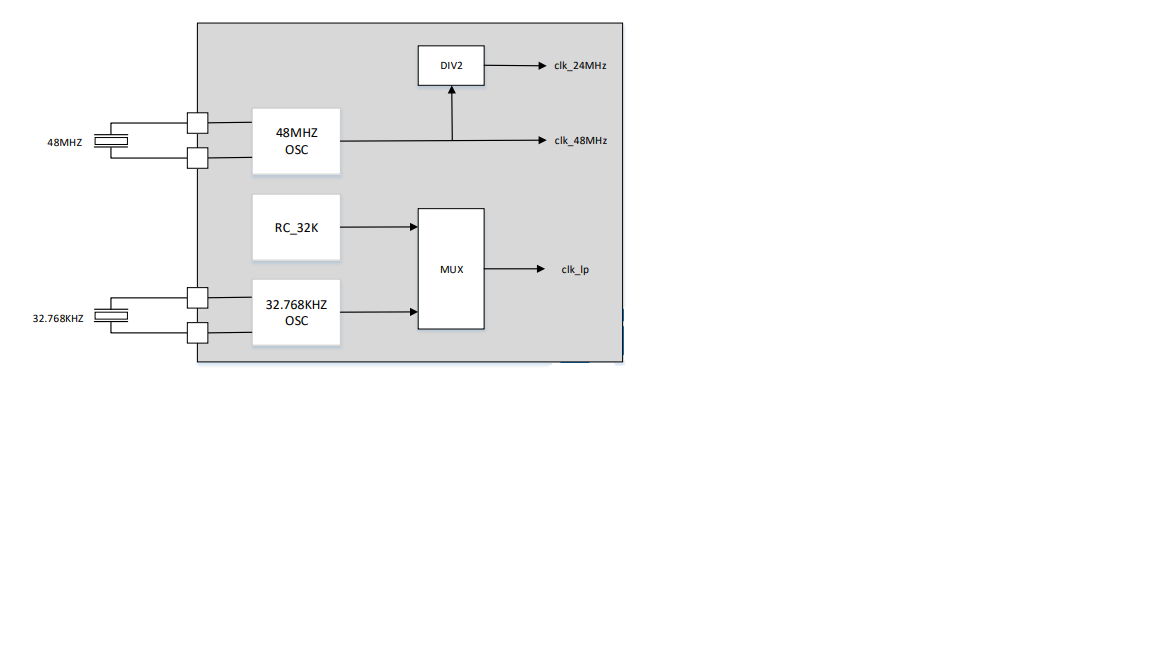
\includegraphics{images/time_structure.png}

\hypertarget{ux4f7fux7528ux8bf4ux660e-2}{%
\section{使用说明}\label{ux4f7fux7528ux8bf4ux660e-2}}

\hypertarget{ux5916ux8bbeux590dux4f4d}{%
\subsection{外设复位}\label{ux5916ux8bbeux590dux4f4d}}

通过 \texttt{SYSCTRL\_ResetBlock} 复位外设,通过'SYSCTRL\_ReleaseBlock'释放复位。

\begin{Shaded}
\begin{Highlighting}[]
\DataTypeTok{void}\NormalTok{ SYSCTRL_ResetBlock(SYSCTRL_ResetItem item);}
\DataTypeTok{void}\NormalTok{ SYSCTRL_ReleaseBlock(SYSCTRL_ResetItem item);}
\end{Highlighting}
\end{Shaded}

\hypertarget{ux65f6ux949fux95e8ux63a7}{%
\subsection{时钟门控}\label{ux65f6ux949fux95e8ux63a7}}

通过 \texttt{SYSCTRL\_SetClkGateMulti} 设置门控(即关闭时钟),通过 \texttt{SYSCTRL\_ClearClkGateMulti} 消除门控(即恢复时钟)。

\begin{Shaded}
\begin{Highlighting}[]
\DataTypeTok{void}\NormalTok{ SYSCTRL_SetClkGateMulti(SYSCTRL_ClkGateItem item);}
\DataTypeTok{void}\NormalTok{ SYSCTRL_ClearClkGateMulti(SYSCTRL_ClkGateItem item);}
\end{Highlighting}
\end{Shaded}

\texttt{SYSCTRL\_SetClkGateMulti} 和 \texttt{SYSCTRL\_ClearClkGateMulti} 可以同时控制多个外设的门控。 \texttt{items} 参数里的各个比特与 \texttt{SYSCTRL\_ClkGateItem} 里的各个外设一一对应。

\begin{Shaded}
\begin{Highlighting}[]
\DataTypeTok{void}\NormalTok{ SYSCTRL_SetClkGateMulti(}\DataTypeTok{uint32_t}\NormalTok{ items);}
\DataTypeTok{void}\NormalTok{ SYSCTRL_ClearClkGateMulti(}\DataTypeTok{uint32_t}\NormalTok{ items);}
\end{Highlighting}
\end{Shaded}

\hypertarget{ux65f6ux949fux914dux7f6e}{%
\subsection{时钟配置}\label{ux65f6ux949fux914dux7f6e}}

举例如下。

\begin{enumerate}
\def\labelenumi{\arabic{enumi}.}
\item
  开启I2C时钟

  使用 \texttt{SYSCTRL\_SelectI2sClk} 为 I2C 配置时钟:

\begin{Shaded}
\begin{Highlighting}[]
\NormalTok{SYSCTRL_ClearClkGateMulti( (}\DecValTok{1}\NormalTok{ << SYSCTRL_ClkGate_APB_I2C0)}
\NormalTok{                          |(}\DecValTok{1}\NormalTok{ << SYSCTRL_ClkGate_APB_PinCtrl));}
\end{Highlighting}
\end{Shaded}
\item
  关闭定时器TMR0时钟

  使用 \texttt{SYSCTRL\_GetClk} 可获得指定外设的时钟频率:

\begin{Shaded}
\begin{Highlighting}[]
\NormalTok{SYSCTRL_ClearClkGateMulti(}\DecValTok{0}
\NormalTok{                        | (}\DecValTok{1}\NormalTok{ << SYSCTRL_ClkGate_APB_TMR0));}
\end{Highlighting}
\end{Shaded}
\end{enumerate}

\hypertarget{timerwatchdog}{%
\chapter{Timer\&Watchdog}\label{timerwatchdog}}

\hypertarget{ux529fux80fdux6982ux8ff0-4}{%
\section{功能概述}\label{ux529fux80fdux6982ux8ff0-4}}

ING918xx系列有三个定时器:\texttt{Timer0}、\texttt{Timer1}和\texttt{Timer2}。三个定时器功能基本相同,可以实现定时、比较等功能。唯一的区别在于,\texttt{Timer0} 可以用作看门狗。

\hypertarget{ux8ba1ux65f6ux5668ux529fux80fd}{%
\subsection{计时器功能}\label{ux8ba1ux65f6ux5668ux529fux80fd}}

用作计时器时,主要实现了以下功能:

\begin{itemize}
\item
  用作32位递增计数器或32位比较器。
\item
  可以设置为普通模式、一次性模式和自由模式:

  \begin{itemize}
  \item
    普通模式(\texttt{TMR\_CTL\_OP\_MODE\_WRAPPING})------计数器以恒定间隔产生中断,在达到比较计数器中的比较值后重置为0,并继续计数,这是默认采用的模式。
  \item
    一次性模式(\texttt{TMR\_CTL\_OP\_MODE\_ONESHOT})------当计数器增长到等于比较器的值时,定时器会禁用,直到下次主动启用它。
  \item
    自由模式(\texttt{TMR\_CTL\_OP\_MODE\_FREERUN})------计数器达到定时器中的值时不会停止,而是会一直递加到最大值(\texttt{0xffffffff}),之后重置为零,并继续计数。
  \end{itemize}
\item
  可以根据设置产生中断。
\end{itemize}

\hypertarget{watchdogux7684ux529fux80fd}{%
\subsection{WATCHDOG的功能}\label{watchdogux7684ux529fux80fd}}

\texttt{Timer0}可以用作看门狗,设定一定的延时时间,在此时间内,如果程序没有主动喂狗,则会发生重启。

看门狗可以在程序跑飞时,让程序复位。

\hypertarget{timerux4f7fux7528ux8bf4ux660e}{%
\section{TIMER使用说明}\label{timerux4f7fux7528ux8bf4ux660e}}

\hypertarget{ux83b7ux53d6timerux8ba1ux6570ux503c}{%
\subsection{获取Timer计数值}\label{ux83b7ux53d6timerux8ba1ux6570ux503c}}

可以通过\texttt{TMR\_GetCNT} 获取计数器的当前计数值。

\begin{verbatim}
uint32_t TMR_GetCNT(TMR_TypeDef *pTMR);
\end{verbatim}

\texttt{pTMR} :可以设置为\texttt{APB\_TMR0}、\texttt{APB\_TMR1}、\texttt{APB\_TMR2},对应\texttt{Timer0}、\texttt{Timer1}和\texttt{Timer2}。

注意计数器只有使能后,计数值才会随着程序的运行递加,如果计数器未使能,计数值是不变的。

\hypertarget{timerux8ba1ux6570ux503cux6e05ux96f6}{%
\subsection{TIMER计数值清零}\label{timerux8ba1ux6570ux503cux6e05ux96f6}}

可以通过\texttt{TMR\_Reload} 将计数器的当前计数值清零。

\begin{verbatim}
void TMR_Reload(TMR_TypeDef *pTMR);
\end{verbatim}

\hypertarget{ux8bbeux7f6etimerux7684ux6bd4ux8f83ux503c}{%
\subsection{设置TIMER的比较值}\label{ux8bbeux7f6etimerux7684ux6bd4ux8f83ux503c}}

可以通过\texttt{TMR\_SetCMP} 设置计数器的比较值。

\begin{verbatim}
void TMR_SetCMP(TMR_TypeDef *pTMR, uint32_t value);
\end{verbatim}

\texttt{pTMR} :选择要设置的计数器,\texttt{APB\_TMR0}、\texttt{APB\_TMR1}或\texttt{APB\_TMR2};

\texttt{value} :设置的比较值。

\hypertarget{ux83b7ux53d6timerux7684ux6bd4ux8f83ux503c}{%
\subsection{获取TIMER的比较值}\label{ux83b7ux53d6timerux7684ux6bd4ux8f83ux503c}}

使用\texttt{TMR\_GetCMP} 获取计数器的比较值;

\begin{verbatim}
uint32_t TMR_GetCMP(TMR_TypeDef *pTMR);
\end{verbatim}

\hypertarget{ux4f7fux80fdtimer}{%
\subsection{使能TIMER}\label{ux4f7fux80fdtimer}}

通过\texttt{TMR\_Enable} 使能计数器。

\begin{verbatim}
void TMR_Enable(TMR_TypeDef *pTMR);
\end{verbatim}

计数器使能之后,计数值才会随着时钟的运行递增。

\hypertarget{ux7981ux80fdtimer}{%
\subsection{禁能TIMER}\label{ux7981ux80fdtimer}}

通过\texttt{TMR\_Disable} 禁能计数器。

\begin{verbatim}
void TMR_Disable(TMR_TypeDef *pTMR);
\end{verbatim}

\hypertarget{ux8bbeux7f6etimerux7684ux5de5ux4f5cux6a21ux5f0f}{%
\subsection{设置TIMER的工作模式}\label{ux8bbeux7f6etimerux7684ux5de5ux4f5cux6a21ux5f0f}}

通过\texttt{TMR\_SetOpMode} 设置计数器的工作模式。

\begin{verbatim}
void TMR_SetOpMode(TMR_TypeDef *pTMR, uint8_t mode);
\end{verbatim}

三种模式的定义如下:

\begin{verbatim}
#define TMR_CTL_OP_MODE_WRAPPING            0
#define TMR_CTL_OP_MODE_ONESHOT             1
#define TMR_CTL_OP_MODE_FREERUN             2
\end{verbatim}

具体说明见\protect\hyperlink{function}{上文}。

\hypertarget{ux4f7fux80fdtimerux4e2dux65ad}{%
\subsection{使能TIMER中断}\label{ux4f7fux80fdtimerux4e2dux65ad}}

通过\texttt{TMR\_IntEnable} 使能中断,使能中断后计时器计数值达到比较值后,会触发中断。

\begin{verbatim}
void TMR_IntEnable(TMR_TypeDef *pTMR);
\end{verbatim}

\hypertarget{ux7981ux80fdtimerux4e2dux65ad}{%
\subsection{禁能TIMER中断}\label{ux7981ux80fdtimerux4e2dux65ad}}

通过\texttt{TMR\_IntDisable}禁能计数器的中断。

\begin{verbatim}
void TMR_IntDisable(TMR_TypeDef *pTMR);
\end{verbatim}

\hypertarget{ux6e05ux9664timerux4e2dux65adux8bf7ux6c42}{%
\subsection{清除TIMER中断请求}\label{ux6e05ux9664timerux4e2dux65adux8bf7ux6c42}}

通过\texttt{TMR\_IntDisable} 清除计数器的中断请求。注意,进入中断处理函数之后,要第一时间清除中断请求,不然可能会重复触发中断。

\begin{verbatim}
void TMR_IntDisable(TMR_TypeDef *pTMR);
\end{verbatim}

\hypertarget{ux83b7ux5f97timerux7684ux4e2dux65adux72b6ux6001}{%
\subsection{获得TIMER的中断状态}\label{ux83b7ux5f97timerux7684ux4e2dux65adux72b6ux6001}}

通过\texttt{TMR\_IntHappened} 来获取计数器的中断状态。

\begin{verbatim}
uint8_t TMR_IntHappened(TMR_TypeDef *pTMR);
\end{verbatim}

\hypertarget{timerux4e2dux65adux4f7fux7528ux6d41ux7a0b}{%
\section{TIMER中断使用流程}\label{timerux4e2dux65adux4f7fux7528ux6d41ux7a0b}}

\begin{itemize}
\item
  配置对应\texttt{Timer}的时钟,下面的代码中配置了三个\texttt{Timer}的时钟,使用时可以根据自己使用的\texttt{Timer}进行配置。

\begin{verbatim}
SYSCTRL_ClearClkGateMulti( (1 << SYSCTRL_ClkGate_APB_TMR0)

                                   | (1 << SYSCTRL_ClkGate_APB_TMR1)

                         | (1 << SYSCTRL_ClkGate_APB_TMR2));
\end{verbatim}
\item
  对\texttt{Timer}进行初始化,以\texttt{Timer1}为例。

\begin{verbatim}
    TMR_SetCMP(APB_TMR1, TMR_CLK_FREQ);
    TMR_SetOpMode(APB_TMR1, TMR_CTL_OP_MODE_WRAPPING);
    TMR_Reload(APB_TMR1);
    TMR_IntEnable(APB_TMR1);
\end{verbatim}

  上面四条语句分别设置了定时器的比较值,设置工作模式,将定时器的当前计数值清零,并使能中断。
\item
  注册中断处理函数。

\begin{verbatim}
platform_set_irq_callback(PLATFORM_CB_IRQ_TIMER1, hr_timer1_isr, NULL);
\end{verbatim}

  \texttt{hr\_timer1\_isr}为\texttt{Timer1}的中断处理函数。
\item
  编写中断处理函数。

\begin{verbatim}
uint32_t hr_timer1_isr(void *user_data)
{
    TMR_IntClr(APB_TMR1);
    //user code
    return 0;
}
\end{verbatim}

  需要注意,中断处理函数中,要优先清理对应的中断请求。
\end{itemize}

\hypertarget{watchdogux4f7fux7528ux8bf4ux660e}{%
\section{Watchdog使用说明}\label{watchdogux4f7fux7528ux8bf4ux660e}}

看门狗(\texttt{Watchdog} )与\texttt{Timer0} 共用一套计数器,看门狗没有使能时,\texttt{Timer0} 与\texttt{Timer1} 、\texttt{Timer2}的使用没有区别,当看门狗使能时,\texttt{Timer0}就不再起作用。

\hypertarget{ux4f7fux80fdux770bux95e8ux72d7}{%
\subsection{使能看门狗}\label{ux4f7fux80fdux770bux95e8ux72d7}}

通过\texttt{TMR\_WatchDogEnable}使能看门狗。

\begin{verbatim}
void TMR_WatchDogEnable(uint32_t timeout);
\end{verbatim}

\texttt{timeout}:设置看门狗的超时时间。

\hypertarget{ux505cux7528ux770bux95e8ux72d7}{%
\subsection{停用看门狗}\label{ux505cux7528ux770bux95e8ux72d7}}

通过\texttt{MR\_WatchDogDisable}禁能看门狗。

\begin{verbatim}
void TMR_WatchDogDisable(void);
\end{verbatim}

\hypertarget{ux5582ux72d7}{%
\subsection{喂狗}\label{ux5582ux72d7}}

通过\texttt{TMR\_WatchDogRestart} 定期喂狗,如果没有在看门狗的超时之前喂狗,程序会发生重启。

这种情况下发生的重启仅能通过硬件重置(\texttt{POR}或者\texttt{RESETN})清除,在其他复位条件下不会清除,可以帮助启动程序检查最近一次复位发生的原因。

  \bibliography{book.bib,packages.bib}

\backmatter
\printindex

\end{document}
